\documentclass{../industrial-development}
\graphicspath{{01-requirement-elicitation/}}

\title{Извлечение требований к ПО}
\author{Петрова Елена Сергеевна, ПИ-21 МО}
\date{}

\begin{document}

\begin{frame}
  \titlepage
\end{frame}
%%%%%%%%%%%%%%%%%%%%%%%%%%%%%%%%%%%%%%%%%%%%%%
\section{Понятие требования}
% 1 слайд
\begin{frame} \frametitle{Понятие требования}
  \begin{block}{}
   \alert{Требование} – это условие или
возможность, которой должна
соответствовать система.
  \end{block}
  Определение IEEE:  \alert{Требование} – это\dots
	 \begin{enumerate}
\item условия или возможности, необходимые
пользователю для решения проблем или
достижения целей;
\item условия или возможности, которыми должна
обладать система или системные
компоненты, чтобы выполнить контракт или
удовлетворять стандартам, спецификациям
или другим формальным документам;
\item документированное представление условий
или возможностей для пунктов 1 и 2.
  \end{enumerate}
\end{frame}

\lecturenotes

Одна из проблем, существующих в индустрии программного обеспечения, — это отсутствие общепринятых определений терминов, которыми мы пользуемся для описания нашей работы. Разные эксперты, говоря об одном и том же документе, называют его и требования пользователя, и требования к ПО, и функциональные требования, и системные требования, и технологические требования, и бизнес-требования, и требования к продукту. Заказчики зачастую считают, что требования -- это развитая концепция продукта, предназначенная для
разработчиков. Те, в свою очередь, полагают, что в отношении клиентов это детальная разработка интерфейса пользователя~\cite[с.~6]{Wiegers}. Такое многообразие ведет к проблемам коммуникации между Заказчиком и Разработчиком.

Определение IEEE Standard Glossary
of Software Engineering Terminology (1990) охватывает требования как пользователей (внешнее поведение системы), так и разработчиков (некоторые скрытые параметры). Термин пользователи следует распространить на всех заинтересованных лиц, так как не все, кто заинтересован в проекте — пользователи~\cite[с.~7]{Wiegers}. 

%%%%%%%%%%%%%%%%%%%%%%%%%%%%%%%%%%%%%%%%%%%%%%%%%%%
\section{Источники требований}
% 2 слайд
\begin{frame} \frametitle{Источники требований }
 \begin{itemize}
\item федеральное и муниципальное отраслевое законодательство (конституция, законы, распоряжения);
\item нормативное обеспечение организации (регламенты, положения, уставы, приказы);
\item текущая организация деятельности объекта автоматизации;
\item модели деятельности (диаграммы бизнес-процессов);
\item представления и ожидания потребителей и пользователей системы;
\item журналы использования существующих программно-аппаратных систем;
\item конкурирующие программные продукты.
  \end{itemize}
Необходимо идентифицировать \alert{все возможные источники требований}, значимые для решения задач проекта. 
\end{frame}

\lecturenotes

Основным источником требований к ПО, безусловно, являются соображения, высказанные представителями Заказчика. Проблема состоит в том, что требования формулируются к создаваемой, ещё не существующей системе, т.е. по сути, решается начальная подзадача задачи проектирования ПО, а представители Заказчика далеко не всегда бывают компетентны в данном вопросе. 

Поэтому, наряду с требованиями, высказанными Заказчиком, целесообразно собирать и требования от других совладельцев системы: сотрудников аналитической группы исполнителя, внешних экспертов и т.д.

Модель создаваемой информационной системы в определённой мере должна отражать модель ОС. Поэтому другим важным источником информации, помимо выявления требований, являются артефакты, описывающие предметную область. Это могут быть документы с описанием бизнес-процессов предприятия, выполненные консалтинговым агентством, либо просто документы (должностные инструкции, распоряжения, своды бизнес-правил), принятые на предприятии.

Ещё одна альтернатива, используемая при выявлении требований – так называемые «лучшие практики», широко используемые в настоящее время в бизнес-консалтинге и при внедрении корпоративных информационных систем. Лучшие практики представляют собой описания моделей деятельности успешных компаний отрасли, используемые длительное время в сотнях и тысячах компаний по всему миру.

Подытоживая сказанное, отметим, что основными источниками, образующими «вход» процесса выявления требований, являются требования, высказанные совладельцами, как таковые или (и) артефакты, описывающие объект исследования.

Однако, это – достаточно упрощённый взгляд: чтобы данные поступили «на вход», аналитики требований должны проделать немалую работу, связанную с подбором респондентов и информационных материалов, организацией интервью и т.д~\cite[с.~29--30]{Maglinec}.

%%%%%%%%%%%%%%%%%%%%%%%%%%%%%%%%%%%%%%%%%%%%%%%%%%%
% 3 слайд
\section{Классификация требований}
\begin{frame} \frametitle{Классификация требований}
 \centerline{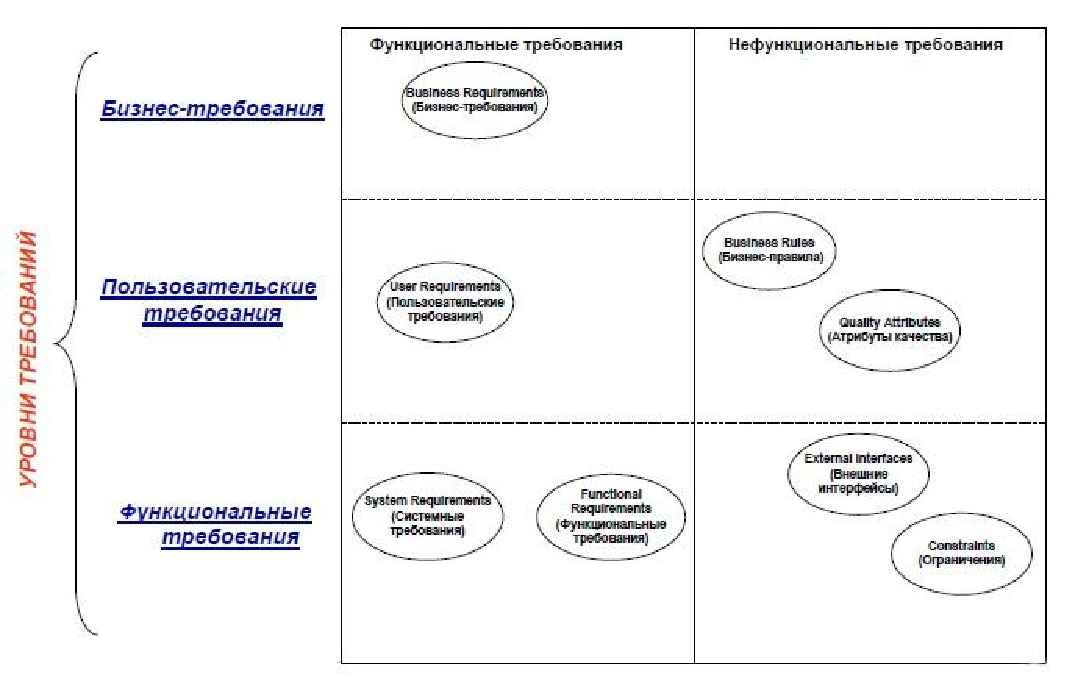
\includegraphics[width=0.9\textwidth]{pict1.pdf}}
\end{frame}

\lecturenotes

Требования к ПО состоят из трех уровней —
бизнес-требования, требования пользователей и функциональные требования. К тому же каждая система имеет свои нефункциональные требования.

%%%%%%%%%%%%%%%%%%%%%%%%%%%%%%%%%%%%%%%%%%%%%%%%%%%
\subsection{Уровни требований}
% 4 слайд
\begin{frame} \frametitle{Уровни требований}
  \begin{block}{}
\alert{Бизнес-требования (Business Requirements)}	содержат высокоуровневые цели организации или заказчиков системы.
  \end{block}
   \begin{itemize}
\item Их высказывают те, кто финансируют проект, покупатели системы, отдел маркетинга.
\item Почему организации нужна такая система? Какие цели организация намерена достичь с ее помощью?
\end{itemize}
  \begin{block}{}
\alert{Требования пользователей (User Requirements)} описывают цели и задачи, которые пользователям позволит решить система. 
    \end{block}
		\begin{itemize}
	\item Способы представления: варианты использования, сценарии и таблицы «событие — отклик». 
	\item Что клиенты смогут делать с помощью системы?
  \end{itemize}
\end{frame}

\lecturenotes

\alert{Бизнес-требования (Business Requirements)} содержат высокоуровневые цели организации или заказчиков системы. Как правило, их высказывают те, кто финансируют проект, покупатели системы, менеджер реальных пользователей, отдел маркетинга или «ясновидец» (специалист по системам машинного зрения). В этом документе объясняется, почему организации нужна такая система, то есть описаны цели, которые организация намерена достичь с ее помощью. Обычно бизнес-требования записываются в форме документа об образе и границах проекта, который еще называют уставом проекта (project charter) или документом рыночных требований (market requirements document).
Определение границ проекта представляет собой первый этап управление общими проблемами расползания границ~\cite[с.~7]{Wiegers}.

Менеджеры и сотрудники отдела маркетинга определяют бизнес-требовния для ПО, чтобы они помогли их компании работать эффективнее (для информационных систем) или успешно конкурировать на рынке (для коммерческих продуктов)~\cite[с.~11]{Wiegers}.

\alert{Требования пользователей (User Requirements)} описывают цели и задачи, которые пользователям позволит решить система. К отличным способам представления этого вида требований относятся варианты использования, сценарии и таблицы «событие — отклик». Таким образом, в этом документе указано, что клиенты смогут делать с помощью системы. Пример варианта использования — заказа билетов на самолет, аренды автомобиля, заказа гостиницы через Интернет~\cite[с.~8--9]{Wiegers}.

На основе требований пользователя аналитики определяют функции, которые позволят пользователям выполнять их задачи~\cite[с.~11]{Wiegers}.

%%%%%%%%%%%%%%%%%%%%%%%%%%%%%%%%%%%%%%%%%%%%%%%%
% 5 слайд
\begin{frame} \frametitle{Уровни требований}
  \begin{block}{}
\alert{Функциональные требования (Functional Requirements)}	определяют функциональность ПО, которую разработчики должны построить, чтобы пользователи смогли выполнить свои задачи в рамках бизнес-требований.
  \end{block}
 		\begin{itemize}
\item Они содержат положения с традиционным «должен» или «должна»: «Система должна по электронной почте отправлять пользователю подтверждение о заказе».
		\end{itemize}
\begin{block}{}
\alert{Системные требования (System Requirements)} -- высокоуровневые требования к продукту, которые содержат многие подсистемы, то есть система.
  \end{block}
 		\begin{itemize}
\item Под системой подразумевается программное обеспечение или подсистемы ПО и оборудования.
		\end{itemize}
\end{frame}

\lecturenotes

\alert{Функциональные требования (Functional Requirements)} определяют функциональность ПО, которую разработчики должны построить, чтобы пользователи смогли выполнить свои задачи в рамках бизнес-требований. Иногда именуемые требованиями поведения (behavioral requirements), они содержат положения с традиционным «должен» или «должна»: «Система должна по электронной почте отправлять пользователю подтверждение о заказе». Функциональные требования описывают, что разработчику необходимо реализовать.

Термином \alert{системные требования (System Requirements)} обозначают высокоуровневые требования к продукту, которые содержат многие подсистемы, то есть система (IEEE, 1998с). Говоря о системе, мы подразумеваем программное обеспечение или подсистемы ПО и оборудования. Люди — часть системы, поэтому определенные функции системы могут распространяться и на людей~\cite[с.~9]{Wiegers}.

%%%%%%%%%%%%%%%%%%%%%%%%%%%%%%%%%%%%%%%%%%%%%%%%%%
% 6 слайд
\subsection{Другие типы требований}
\begin{frame} \frametitle{Другие типы требований}
  \begin{block}{}
\alert{Нефункциональные требования (Non Functional Requirements)}	включают эксплуатационные характеристики и описание атрибутов качества.
  \end{block}
	\begin{itemize}
\item \alert{Бизнес-правила (Business Rules)}	включают корпоративные политики, правительственные постановления, промышленные стандарты и вычислительные алгоритмы.
\item \alert{Атрибуты качества (Quality Attributes)} представляют собой дополнительное описание функций продукта, выраженное через описание его характеристик, важных для пользователей или разработчиков.
	\begin{itemize}
	\item Основные атрибуты качества: применимость,  надежность, производительность, эксплуатационная пригодность.
	\end{itemize}
	\end{itemize}
		\end{frame}
		
\lecturenotes

Нефункциональные требования, соответственно, регламентируют внутренние и внешние условия или атрибуты функционирования системы~\cite[с.~10]{Maglinec}.

\alert{Бизнес-правила (Business Rules)} включают корпоративные политики, правительственные постановления, промышленные стандарты и вьчислительные алгоритмы. Бизнес-правила не являются требованиями к ПО, потому что они находятся снаружи границ любой системы ПО. Однако они часто налагают ограничения, определяя, кто может выполнять конкретные варианты использования, или диктовать, какими функциями должна обладать систем, подчиняющаяся соответствующим правилам. Иногда бизнес-правила становятся источником атрибутов качества, которые реализуются в функциональности. Следовательно, мы можем отследить происхождение конкретных функциональных требований вплоть до соответствующих им бизнес-правил~\cite[с.~9]{Wiegers}.

В дополнение к функциональным требованиям спецификация содержит нефункциональные, где описаны цели и атрибуты качества. \alert{Атрибуты качества (Quality Attributes)} представляют собой дополнительное описание функций продукта, выраженное через описание его характеристик, важных для пользователей или разработчиков. К таким
характеристикам относятся легкость и простота использования, легкость перемещения, целостность, эффективность и устойчивость к сбоям~\cite[с.~10]{Wiegers}.

%%%%%%%%%%%%%%%%%%%%%%%%%%%%%%%%%%%%%%%%%%%%%%%%%%%
% 7 слайд
\begin{frame} \frametitle{Другие типы требований}
	\begin{itemize}

\item \alert{Ограничения (Constraints)} -- формулировки условий, модифицирующих требования или наборы требований, сужая выбор возможных решений по их реализации.
\begin{itemize}
	\item Выбор платформы реализации и/или развертывания, протоколы, серверы приложений, баз
данных и т.д.
\end{itemize}
\item К \alert{внешним интерфейсам (External Interfaces)} относятся интерфейс пользователя (User Interface), интерфейсы с внешними устройствами (аппаратные) и программные интерфейсы и интерфейсы передачи информации (коммуникационные интерфейсы).
	\end{itemize}

	\end{frame}

\lecturenotes

Другие нефункциональные требования описывают внешние
взаимодействия между системой и внешним миром, а также ограничения дизайна и реализации. \alert{Ограничения (Constraints)} касаются выбора
возможности разработки внешнего вида и структуры продукта~\cite[с.~10]{Wiegers}.

Среди \alert{внешних интерфейсов} в большинстве современных АИС наиболее важным является интерфейс пользователя (User Interface, UI). Кроме того, выделяются интерфейсы с внешними устройствами (аппаратные интерфейсы), программные интерфейсы и
интерфейсы передачи информации (коммуникационные интерфейсы)~\cite[с.~10]{Maglinec}.

Разработчикам необходимы функциональные и нефункциональные требования, чтобы создавать
решения с желаемой функциональностью, определенным качеством и требуемыми рабочими характеристиками, не выходя за рамки налагаемых ограничений~\cite[с.~11]{Wiegers}.

%%%%%%%%%%%%%%%%%%%%%%%%%%%%%%%%%%%%%%%%%%%%%%
%8 слайд
\begin{frame} \frametitle{Пример разных типов требований}
	\begin{itemize}
	\item \alert{Бизнес-требование}: «Программа подготовки текстов позволит пользователям исправлять орфографические ошибки в тексте эффективно».
	\item \alert{Требования пользователей}: «Найдите орфографическую ошибку», «Добавьте слово в общий словарь».
	\item \alert{Функциональные требования}: поиск и выделение слова с ошибкой, отображение диалогового окна с фрагментом текста, где это слово находится, и замена слова с ошибкой корректным вариантом по всему тексту.
	\item \alert{Атрибут качества} легкость и простота использования (usability) определяет его значение посредством слова «эффективно» в бизнес-требованиях.
	\end{itemize}
\end{frame}

\lecturenotes

Рассмотрим в качестве примера программу подготовки текстов. Бизнес-требование может выглядеть так: «Продукт позволит пользователям исправлять ор-фографические ошибки в тексте эффективно». На коробке CD-ROM указано, что проверка грамматики включена как характеристика, удовлетворяющая бизнес-требования. Соответствующие требования пользователей могут содержать задачи (варианты использования) вроде такой: «Найдите орфографическую ошибку» или «Добавьте слово в общий
словарь». Проверка грамматики имеет множество индивидуальных функциональных требований, которые связаны с такими операциями, как поиск и выделение слова с ошибкой, отображение диалогового окна
с фрагментом текста, где это слово находится, и замена слова с ошибкой корректным вариантом по всему тексту. Атрибут качества легкость и простота использования (usability) как раз и определяет его значение посредством слова «эффективно» в бизнес-требованиях~\cite[с.~10--11]{Wiegers}.


%%%%%%%%%%%%%%%%%%%%%%%%%%%%%%%%%%%%%%%%%%%%%%%
\section{Свойства требований}
% 9 слайд
\begin{frame} \frametitle{Свойства требований}
  \centerline{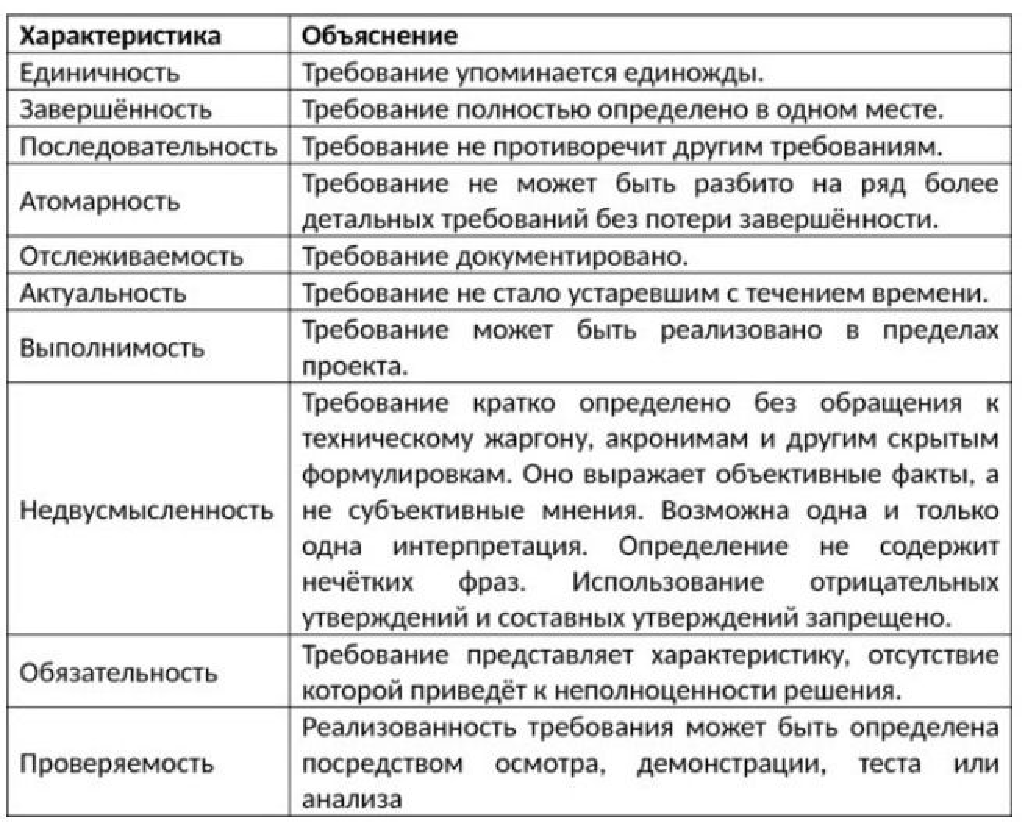
\includegraphics[width=0.9\textwidth]{pict2.pdf}}
\end{frame}

\lecturenotes

В идеальном мире каждое требование отвечает различным параметрам качества, которые и описаны в представленной таблице.

\alert{Полнота/Завершенность}

Каждое требование должно полно описывать функциональность, которую следует реализовать в продукте. То есть оно должно содержать
всю информацию, необходимую для разработчиков, чтобы тем удалось создать этот фрагмент функциональности. Если данных определенного рода не хватает, используется пометка «TBD» (to be determined — необходимо определить) на полях как стандартный флаг для выделения такого места. Необходимо восполнить все пробелы в каждом фрагменте требований, прежде чем приступать к конструированию какой-либо функции.

\alert{Корректность/Последовательность}

Каждое требование должно точно описывать желаемую функциональность. Для соблюдения корректности необходима связь с источниками требований, например, с пожеланиями пользователей или высоко-
уровневыми системными. Требования к ПО, которые конфликтуют с родительскими требованиями, нельзя считать корректными. Однако основная оценка здесь — за представителями пользователей, вот почему им или их непосредственным заместителям необходимо предоставлять требования для просмотра.

\alert{Выполнимость/Осуществимость}

Необходима возможность реализовать каждое требование при известных условиях и ограничениях системы и операционной среды.
Чтобы не столкнуться с недостижимыми положениями, необходимо обеспечить взаимодействие разработчиков с маркетологами и аналитиками требований
на период всего извлечения требований. Разработчики реально оценят, что можно выполнить технически, а что нет, или что сделать можно, но при дополнительном финансировании. Инкрементальная разработка и подтверждающие концепцию прототипы позволяют проверить осуществимость требования.

\alert{Обязательность/Необходимость}

Каждое требование должно отражать возможность, которая действительно необходима пользователям или которая нужна для соответствия внешним системным требованиям или стандартам. Кроме того,
оно должно исходить от лица, которое имеет полномочия на запись положения. Необходимо отслеживать каждое требование вплоть до стадии сбора
мнений пользователей, когда выявляются варианты использовании, бизнес-правила или другие источники.

\alert{Недвусмысленность}

Все читатели требований должны интерпретировать их одинаково, но естественный язык зачастую грешит многозначностью. Описывать документацию следует просто, кратко и точно, применяя лексику, понятную пользователям. «Ясность» — цель качества требований, связанная с точностью: читатели должны четко понимать каждое положение. Все специальные термины рекомендуется заносить в словарь.

\alert{Проверяемость}

Необходимо разрабатывать тесты или применять другие приемы для проверки, например, экспертизу или демонстрации, чтобы
установить, действительно ли в продукте реализовано каждое требование. Если требование не проверяется, вопрос его корректной реализации становится предметом заключения, а не целью анализа. Неполные, несогласованные, невыполнимые или двусмысленные требования также не проверяются (Drabick 1999)~\cite[с.~24]{Wiegers}.

%%%%%%%%%%%%%%%%%%%%%%%%%%%%%%%%%%%%%%%%%%%%%%%%
\section{Разработка требований}
% 10 слайд
\begin{frame} \frametitle{Разработка требований}
  \centerline{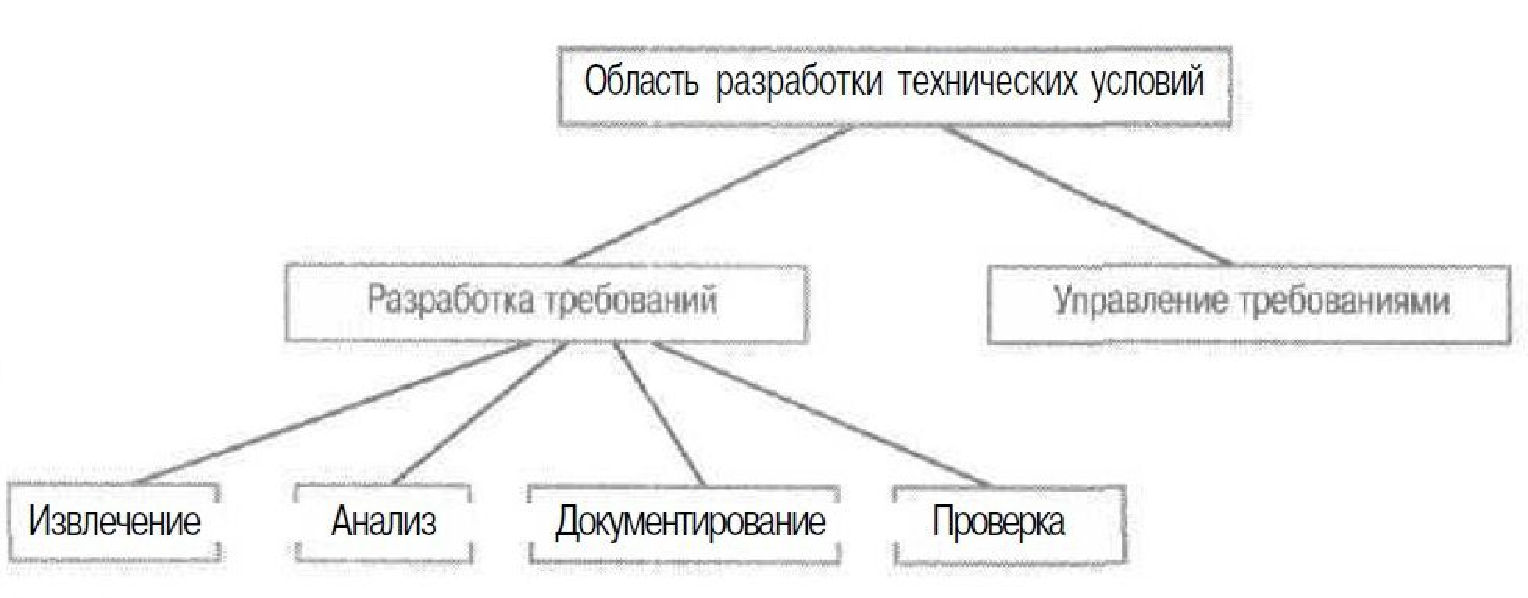
\includegraphics[width=0.9\textwidth]{pict3.pdf}}
\end{frame}

\lecturenotes

 Этап разработки требований можно подразделить на извлечение (elicitation), анализ (analysis), документирование (specification) и утверждение (validation) (Abran и Moore, 2001). В эти подэтапы входят все действия, включающие сбор, оценку и документирование требований для ПО
или ПО-содержащих продуктов, в том числе:
	\begin{itemize}
\item идентификация классов пользователей для данного продукта;
\item выяснение потребностей тех, кто представляет каждый класс пользователей;
\item определение задач и целей пользователей, а также бизнес-целей, с которыми эти задачи связаны;
\item анализ информации, полученной от пользователей, чтобы отделить задачи от функциональных и нефункциональных требований, бизнес-правил, предполагаемых решений и поступающих извне данных;
\item распределение высокоуровневых требований по компонентам ПС, определенным в системной архитектуре;
\item установление относительной важности атрибутов качества;
\item установление приоритетов реализации;
\item документирование собранной информации и построение моделей;
\item просмотр спецификации требований, который позволяет удостовериться в том, что запросы пользователей всеми понимаются одинаково, и устранение возникших проблем до передачи документа разработчикам.
\end{itemize}

Постепенность процесса — ключ к успеху разработки требований. Необходимо планировать цикличность исследования требований, детализировать высокоуровневые требования и уточнять их корректность у пользователей. Выполнение этих задач требует времени, однако это важный аспект работы с неясно определенным новым ПО~\cite[с.~12-13]{Wiegers}.

%%%%%%%%%%%%%%%%%%%%%%%%%%%%%%%%%%%%%%%%%%%%%%%%%%
\subsection{Извлечение требований}
% 11 слайд
\begin{frame} \frametitle{Извлечение требований}
\begin{itemize}

\item \alert{Интервью с потенциальными пользователями и экспертами}
\begin{itemize} 
\item Какие задачи требуется выполнять средствами ПО? 
\item Как должен клиент взаимодействовать с
системой для выполнения каждой задачи? 
\end{itemize}

\item \alert{Анкетирование}
\begin{itemize} 
\item Подготовка и анализ анкет требуют небольшой ресурс.
\item Велика вероятность получить неполную или вовсе ложную информацию. 
\end{itemize}

\item \alert{Наблюдение}
\begin{itemize} 
\item Наблюдая за работой пользователей, выявляют контекст потенциального применения нового продукта.
\item Наблюдатель, как и всякий «измерительный прибор», вносит помехи в результаты измерений.
\end{itemize} 

\end{itemize}
\end{frame}

\lecturenotes

\alert{Работа с пользователями для выяснения назначения продукта}

Необходимо выяснять у пользователей, какие задачи им требуется выполнять средствами ПО. Обсуждать, как должен клиент взаимодействовать с системой для выполнения каждой такой задачи. При 
этом пользуясь стандартным шаблоном для документирования всех задач и для каждой формулировать функциональные требования. Похожий способ, часто применяемый в правительственных проектах, — создание документа с
концепциями операций (ConOps), где указаны характеристики новой системы сточки зрения пользователя (IEEE, 1998a)~\cite[с.~46]{Wiegers}.


\alert{Анкетирование}

Самый малозатратный для аналитика способ извлечения информации, он же – и наименее эффективный. Обычно применяется как дополнение к другим стратегиям выявления требований.
Недостатки анкетирования очевидны: респонденты часто бывают неспособны, либо слабо мотивированы в том, чтобы хорошо и информативно заполнить анкету. Велика вероятность получить неполную или вовсе ложную информацию. Преимущество – в том,
что подготовка и анализ анкет требуют небольшой ресурс~\cite[с.~32]{Maglinec}.

\alert{Наблюдение за пользователями на рабочих местах}

Наблюдая за работой пользователей, выявляют контекст потенциального применения нового продукта (Beyer и Holtzblatt, 1998). Простые диаграммы рабочих потоков, а также диаграммы потоков данных позволяют выяснить, где, как и какие данные задействовал пользователь. Документируя ход бизнес-процесса, удается определить требования к системе
предназначенной для поддержки этого процесса. Иногда даже выясняется, что для выполнения деловых задач клиентам вовсе и не требуется новое ПО (McGraw и Harbison, 1997)~\cite[с.~47]{Wiegers}.

Различают пассивное и активное наблюдение. При активном наблюдении аналитик работает, как участник команды, что позволяет улучшить понимание процессов. Через наблюдение, а возможно, и участие аналитики получают информацию о происходящих день за днем операциях из первых рук. Во время наблюдения за работой системы часто возникают вопросы, которые никогда бы не появились, если бы аналитик только читал документы или разговаривал с экспертами.

Недостатком этой стратегии является то, что наблюдатель, как и всякий «измерительный прибор», вносит помехи в результаты измерений: сотрудники
организации, находясь «под колпаком» могут начать вести себя принципиально по-другому, чем обычно~\cite[с.~32]{Maglinec}.

%%%%%%%%%%%%%%%%%%%%%%%%%%%%%%%%%%%%%%%%%%%%%%%%%
% 12 слайд
\begin{frame} \frametitle{Извлечение требований}
\begin{itemize}

\item \alert{Самостоятельное описание требований}
\begin{itemize} 
\item Чтение и анализ документов - прекрасный способ получить первоначальное представление о системе и сформулировать вопросы к экспертам.
\item Опасность пропуска знаний, специфичных для объекта исследования, либо неформализованных знаний, эмпирических правил и процедур, широко используемых на практике, но не вошедших в документы.
\end{itemize}

\item \alert{Совместные семинары}
\begin{itemize} 
\item Позволяет наладить связи между пользователями и разработчиками.
\item Примеры таких семинаров — Joint Requirements Planning (JRP — совместное планирование требований)и Joint Application Development (JAD — совместная разработка приложений).
\end{itemize}

\end{itemize}
\end{frame}
\lecturenotes

\alert{Самостоятельное описание требований}

Чтение документов - прекрасный способ получить первоначальное представление о системе и сформулировать вопросы к экспертам. Если опытный аналитик уже исследовал большое число систем такого же типа, что и на предприятии внедрения, он обладает фундаментальными знаниями в соответствующей предметной области, относительно определенного класса систем.

По результатам анализа документов и собственных знаний аналитик может составить описание требований и предложить его представителям Заказчика в качестве информации к размышлению, либо – основы для формирования технического задания.

Недостаток этой стратегии – опасность пропуска знаний, специфичных для объекта исследования (в случае самоопроса), либо – неформализованных знаний, эмпирических правил и процедур, широко используемых на практике, но не вошедших в документы~\cite[с.~33]{Maglinec}.

\alert{Изучение отчетов о проблемах работающих систем с целью поиска новых идей}

Поступающие от клиентов отчеты о проблемах и
предложения о расширении функциональности — отличный источник идей о возможностях, которые можно реализовать в следующей версии или новом продукте. За подобной информацией стоит обратиться
и к персоналу службы поддержки~\cite[с.~48]{Wiegers}.

\alert{Проведение совместных семинаров}

Совместные семинары по выявлению требований, где тесно сотрудничают аналитики и клиенты —
отличный способ выявить нужды пользователей и составить наброски документов с требованиями (Gottesdiener, 2002). Конкретные примеры таких семинаров — Joint Requirements Planning (JRP — совместное планирование требований) (Martin, 1991) и Joint Application Development (JAD — совместная разработка приложений) (Wood и Silver, 1995)~\cite[с.~47]{Wiegers}.

%%%%%%%%%%%%%%%%%%%%%%%%%%%%%%%%%%%%%%%%%%%%%
% 13 слайд
\begin{frame} \frametitle{Методы извлечения требований}
Участники JAD-совещания:
  \begin{itemize} 
\item \alert{Ведущий} – специалист в области межличностных коммуникаций. Должен
ориентироваться в предметной области, но не обязательно хорошо ориентироваться в
проблемах IT.
\item \alert{Секретарь} – стенографист встречи, фиксирующий её результаты. Возможно применение CASE-средств.
\item \alert{Заказчики} – пользователи или руководители; основные участники, формирующие,
обсуждающие требования и принимающие решения.
\item \alert{Разработчики} – аналитики и другие участники проектной команды. Работают в
большей части в пассивном режиме с целью лучшего понимания проблемной области.
\end{itemize}
\end{frame}

\lecturenotes

Помимо классического интервью «тет а тет», существует значительное количество
методик, предполагающих широкое участие представителей Заказчика и Исполнителя.
Правила мозгового штурма предполагают полную раскрепощённость и свободу мнений. 
Затем, на втором этапе, все высказанные мнения тщательным образом обсуждаются, заведомо неприемлемые варианты отсеиваются, формируются
коллективные предложения.

Правила JAD-метода, считающегося одним из современных способов извлечения
требований, были впервые сформулированы в конце 1970-х годов компанией IBM.

Участники JAD-совещания:

\alert{Ведущий} – специалист в области межличностных коммуникаций. Должен
ориентироваться в предметной области, но не обязательно хорошо ориентироваться в
проблемах IT.

\alert{Секретарь} – стенографист встречи, фиксирует её результаты. Возможно применение CASE-средств.

\alert{Заказчики} – пользователи или руководители, основные участники, формирующие,
обсуждающие требования и принимающие решения.

\alert{Разработчики} – аналитики и другие участники проектной команды. Работают в
большей части в пассивном режиме с целью наилучшего понимания проблемной области.

Совместные семинары, сохраняя все преимущества режима интервью, привносят дополнительные бонусы: работа в группе более продуктивна, группы быстрее обучаются, более склонны к квалифицированным заключениям, позволяют исключить многие
ошибки. Эта стратегия, очевидно, одна из самых затратных, однако она окупается за счёт
меньшего количества ошибок и отказе от формализации в пользу живого общения,
выработке общего языка и пр~\cite[с.~33]{Maglinec}.


%%%%%%%%%%%%%%%%%%%%%%%%%%%%%%%%%%%%%%%%%%%%
% 14 слайд
\begin{frame} \frametitle{Методы извлечения требований}
   
\begin{itemize}
\item \alert{Метод RAD} – один из наиболее известных способов быстро создавать прототипы.
\item RAD базируется на следующих базовых принципах:
\begin{enumerate}
\item Эволюционное прототипирование;
\item CASE-средства, как основной инструмент, включая возможности прямого и
обратного проектирования и автоматической генерации кода;
\item  Высококвалифицированные специалисты, хорошо владеющие развитыми инструментальными средствами;
\item Интерактивный JAD-метод, в котором общение совмещается с разработкой в режиме online;
\item Жёсткие временные рамки, как противоядие от «расползания границ» проекта: если команда не укладывается в срок – функционал сужается.
\end{enumerate}
\end{itemize}

\end{frame}
\lecturenotes

Прототипирование – ключевая стратегия выявления и проверки требований в большинстве современных методологий. Программный прототип –
«зеркало», в котором видно отражение того, как понял Исполнитель требования Заказчика. 

Документальный способ выявления требований
всегда уступает живому общению. Анализ того, что сделано в виде интерфейсов пользователя даёт ещё больший эффект. 

Метод RAD – один из наиболее известных способов быстро создавать прототипы.

RAD базируется на следующих базовых принципах:
\begin{enumerate}
\item Эволюционное прототипирование.
\item CASE-средства, как основной инструмент, включая возможности прямого и
обратного проектирования и автоматической генерации кода.
\item Высококвалифицированные специалисты, хорошо владеющие развитыми
инструментальными средствами.
\item Интерактивный JAD-метод, в котором общение совмещается с разработкой
в режиме online.
\item Жёсткие временные рамки, как противоядие от «расползания границ» проекта: если команда не укладывается в срок – функционал сужается~\cite[с.~33--34]{Maglinec}.
\end{enumerate}



%%%%%%%%%%%%%%%%%%%%%%%%%%%%%%%%%%%%%%%%%%%%%%
\subsection{Анализ требований}
% 15 слайд
\begin{frame} \frametitle{Анализ требований}
  \begin{block}{}
   \alert{Анализ требований} - их детализация, гарантирующая, что требования понимают все заинтересованные лица, а также тщательное исследование требований на предмет ошибок, пробелов и других недостатков.
  \end{block}

	
\begin{itemize}

\item \alert{Создание контекстной диаграммы} 

\begin{itemize}
\item Контекстная диаграмма — простая модель анализа, отображающая место новой системы в соответствующей среде.
\end{itemize}

\item \alert{Создание пользовательского интерфейса и технических прототипов} 

\begin{itemize}
\item Прототип — частичая, возможная или предварительная версия продукта, которая сделает концепции и возможности более осязаемыми. 1- с.48
\end{itemize}

\end{itemize}

\end{frame}

\lecturenotes

Для того, чтобы повысить уровень информативности требований, устранить взаимные противоречия и добиться выполнения их других основных характеристик,
осуществляется переход от полностью неформализованных текстов к частично
регламентированным (например, шаблонами MS Word) текстам, классификация,
присвоение наборов атрибутов, построение моделей, прототипирование~\cite[с.~40]{Maglinec}.

\alert{Создание контекстной диаграммы}

Контекстная диаграмма — простая модель анализа, отображающая место новой системы в соответствующей среде. Она определяет границы и интерфейсы между разрабатываемой системой и сущностями, внешними для этой системы, например пользователями, устройствами и прочими информационными системами~\cite[с.~48]{Wiegers}.

\alert{Создание пользовательского интерфейса и технических прототипов}

Если разработчики или пользователи не совсем уверены насчет требований, создается прототип — частичная, возможня или предварительная версия продукта, которая сделает концепции и возможности более осязаемыми. Оценка прототипа поможет всем заинтересованным лицам достичь взаимопонимания по решаемой проблеме~\cite[с.~48]{Wiegers}.


%%%%%%%%%%%%%%%%%%%%%%%%%%%%%%%%%%%%%%%%%%%%%%%%%%
% 16 слайд
\begin{frame} \frametitle{Методы анализа требований}
\begin{itemize}
\item  \alert{Анализ осуществимости требований} 
\begin{itemize}
\item Насколько реально реализовать каждое требование при разумных затратах и с приемлемой производительностью в предполагаемой среде.
\end{itemize}
\item \alert{Определение приоритетов требований} 
\begin{itemize}
\item В ходе работы над проектом периодически нужна корректировка приоритетов
в соответствии с потребностями клиента, условиями рынка и бизнес-целями.
\end{itemize}
\item \alert{Моделирование требований} 
\begin{itemize}
\item Диаграммы потоков данных, диаграммы «сущность — связь», диаграммы перехода состояний, карты диалогов, диаграммы классов, диаграммы последовательностей, диаграммы взаимодействий, таблицы решений и деревья решений.
\end{itemize}
\end{itemize}
\end{frame}

\lecturenotes

\alert{Анализ осуществимости требований}

Необходимо анализировать, насколько реально реализовать каждое требование при разумных затратах и с приемлемой производительностью в предполагаемой среде. Рассмотреть риски, связанные с реализацией каждого требования, включая конфликты с другими требованиями, зависимость от внешних факторов и препятствия технического характера~\cite[с.~48]{Wiegers}.

\alert{Определение приоритетов требований}

Пользуясь аналитическим подходом, определяют относительные приоритеты реализации функций продукта, решаемых задач или отдельных требований.
На основании приоритетов установливается, в какой версии будет реализована та или иная функция или набор требований. Подтверждая изменения, все они распределяются по конкретным версиям, в план выпуска включаются затраты необходимые на внесение изменений.
В ходе работы над проектом периодически корректируются приоритеты в соответствии с потребностями клиента, условиями рынка и бизнес-
целями~\cite[с.~48-49]{Wiegers}.

\alert{Моделирование требований}

В отличие от подробной информации, представленной в спецификации требований к ПО или пользователь-
ского интерфейса прототипа, графическая модель анализа отображает требования на высоком уровне абстракции. Модели позволяют выявить некорректные, несогласованные, отсутствующие и избыточные
требования. К таким моделям относятся диаграммы потоков данных, диаграммы «сущность — связь», диаграммы перехода состояний, называемые также автоматами (statecharts), карты диалогов, диаграммы
классов, диаграммы последовательностей, диаграммы взаимодействий, таблицы решений и деревья решений~\cite[с.~49]{Wiegers}.

%%%%%%%%%%%%%%%%%%%%%%%%%%%%%%%%%%%%%%%%%%%%%%%
\begin{frame} \frametitle {Диаграмма вариантов использования}
 \centerline{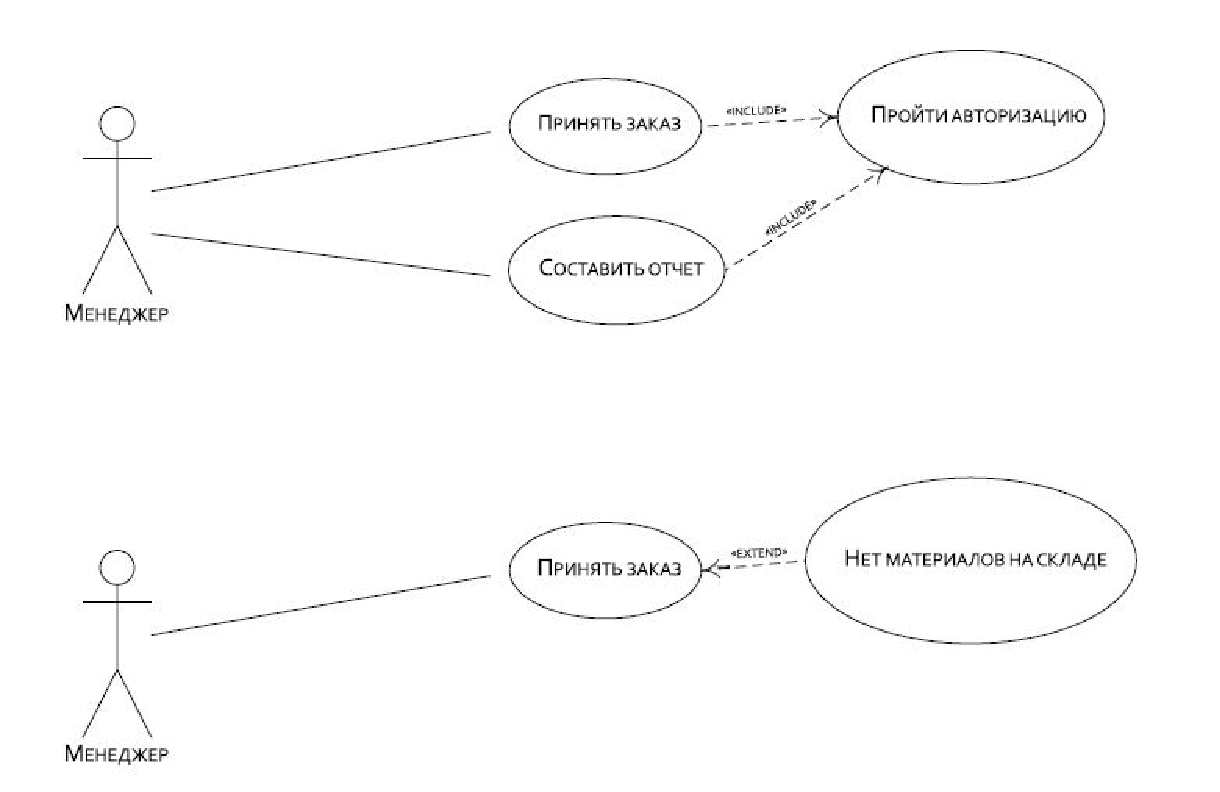
\includegraphics[width=0.8\textwidth]{pict4.pdf}}
\end{frame}

\lecturenotes

\alert{Диаграмма вариантов использования UML, Use Case Diagram} – одно из самых простых представлений системы. Её базовые «строительные элементы» – акторы и варианты использования. Диаграмма задумана так, чтобы дать наиболее общее
представление о функциональности системы (её компоненты), не вдаваясь в детали
взаимосвязей функций. Поэтому основной вид отношения, используемый в диаграмме –
ассоциация между актором и вариантом использования.

Другие виды отношений – отношение включения (include), расширения (extend) и
обобщения/генерализации. Включение служит для обозначения подчинённых вариантов использования (когда один или более вариантов использования содержат вызовы одной и той же
функциональности). Расширение в точности соответствует точке расширения, используемой при
описании варианта использования.

Отношение обобщения может применяться как к акторам, так и к вариантам
использования, с целью указания специализации одних относительно других~\cite[с.~46]{Maglinec}.

%%%%%%%%%%%%%%%%%%%%%%%%%%%%%%%%%%%%%%%%%%%%%%

\begin{frame} \frametitle {Диаграмма действий}
 \centerline{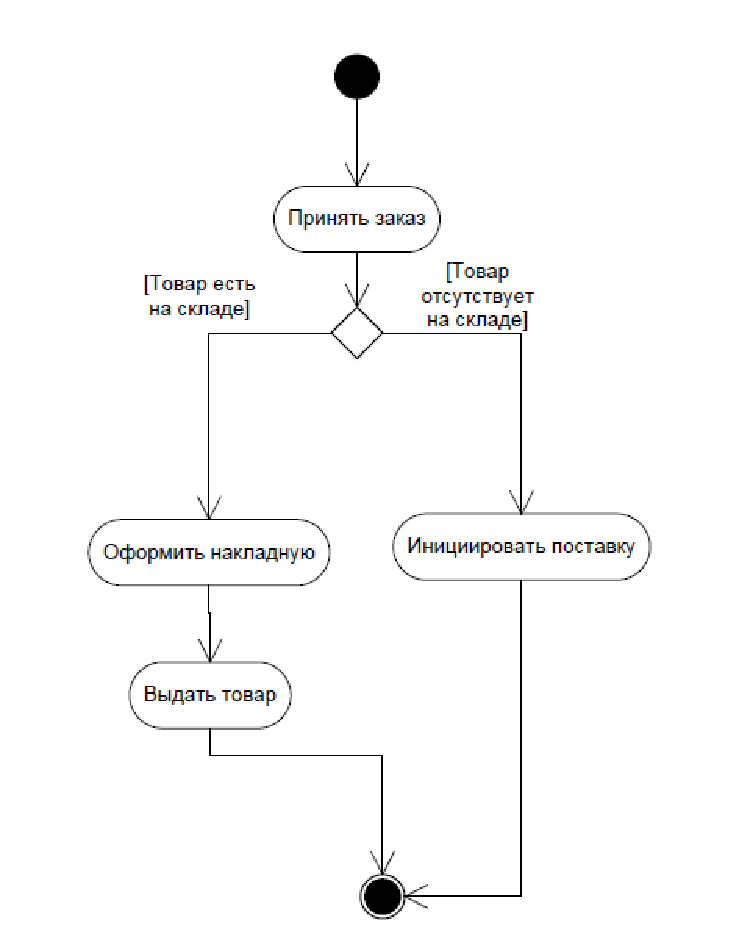
\includegraphics[width=0.6\textwidth]{pict5.pdf}}
\end{frame}

\lecturenotes

Если диаграмма вариантов использования даёт «вид сверху» на функциональность системы, /alert{диаграмма действий UML}, напротив, позволяет подробно иллюстрировать отдельный вариант использования и его сценарии.

Основные компоненты описания системы:
\begin{itemize}
\item функции (действия);
\item символы «старт» и «стоп»;
\item потоки управления;
\item разветвители;
\item линейки синхронизации.
\end{itemize}

Диаграмма действий позволяет проиллюстрировать вариант использования с требуемой степенью подробности. Линейный вариант использования приводит к диаграмме действий с линейным потоком управления между действиями. Действия
варианта использования с альтернативными сценариями реализуется через разветвители.
Линейки синхронизации позволяют описывать такие сложные конструкции, как синхронизацию начала (окончания) параллельных во времени процессов.

Помимо стандартного формата описания, UML предлагает вариант с «плавательными дорожками». Этот формат удобен для описания случая, когда в варианте использования участвуют несколько акторов.
~\cite[с.~47-48]{Maglinec}.

%%%%%%%%%%%%%%%%%%%%%%%%%%%%%%%%%%%%%%%%%%%%%

\begin{frame} \frametitle {Диаграмма состояний}
 \centerline{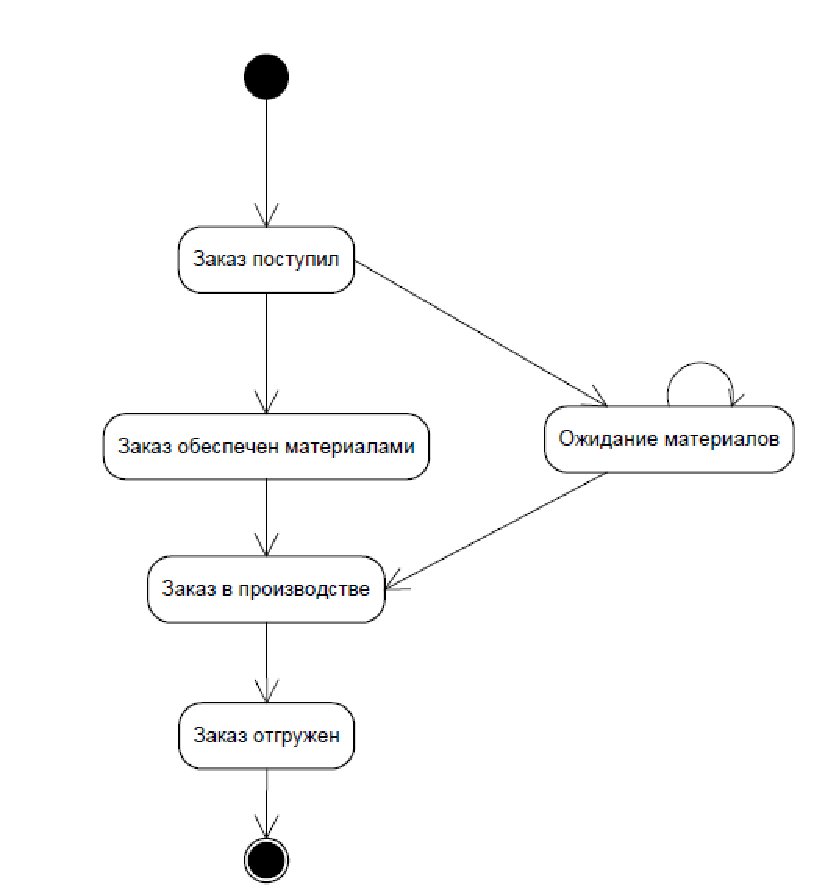
\includegraphics[width=0.7\textwidth]{pict6.pdf}}
\end{frame}

\lecturenotes

\alert{Диаграмма состояний} в анализе требований используется, когда требуется
исследовать поведение системы, как конечного автомата. 

В общем случае диаграмма состояний описывает, как система себя ведёт в более,
чем одном варианте использования. Синтаксис диаграмм состояний во многом совпадает
с синтаксисом диаграмм действий.

Основные компоненты описания системы:
\begin{itemize}
\item простые состояния;
\item составные состояния;
\item символы «старт» и «стоп»;
\item переходы;
\item линейки синхронизации.
\end{itemize}

В языке UML под состоянием понимается абстрактный метакласс, используемый
для моделирования отдельной ситуации, в течение которой имеет место выполнение
некоторого условия. Состояние может быть задано в виде набора конкретных
значений атрибутов класса или объекта, при этом изменение их отдельных значений будет
отражать изменение состояния моделируемого класса или объекта.

Переход системы из состояния в состояние осуществляется при наступлении
событий. При этом говорится, что переход срабатывает. Переход может быть
безальтернативным, либо содержать альтернативы. Во втором случае переход обусловлен
наступлением сторожевых условий. Наконец, событие может сопровождаться
выражением действия, которое происходит в случае, если срабатывает переход. Полный
синтаксис описания перехода (надписи на стрелке) следующий:

\alert{Событие [сторожевое условие] / выражение действия}

Иногда бывает полезным объединить часть состояний в одно мета-состояние.
Графически это выглядит, как символ состояния (прямоугольник со скруглёнными
углами), содержащий внутри себя несколько символов состояний. При этом возможны
переходы между подчинёнными состояниями, переходы между подчинённым и внешним
состояниями и переходы между составным и внешним состоянием~\cite[с.~48-49]{Maglinec}.

%%%%%%%%%%%%%%%%%%%%%%%%%%%%%%%%%%%%%
\begin{frame} \frametitle {Диаграмма потоков данных}
 \centerline{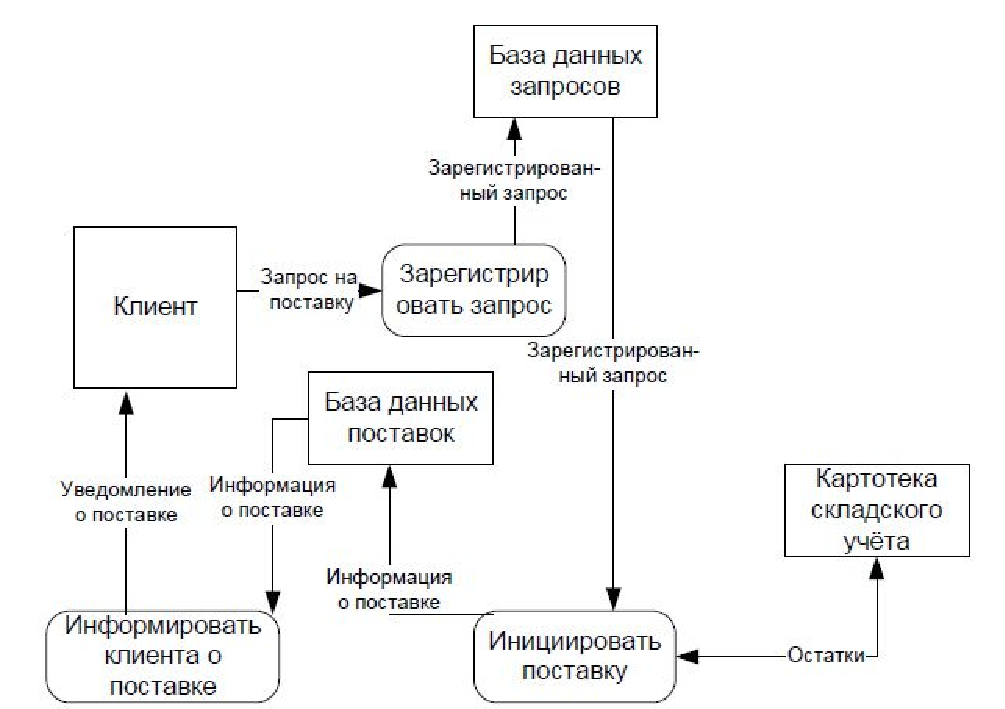
\includegraphics[width=0.8\textwidth]{pict7.pdf}}
\end{frame}

\lecturenotes

\alert{Диаграмма потоков данных} (data flow diagram, DFD) – несмотря на имеющее место в современных условиях смещение акцентов от структурного к объектно-ориентированному подходу к
анализу и проектированию систем, «старинные» структурные нотации по-прежнему
широко и эффективно используются как в бизнес-анализе, так и в анализе
информационных систем.

Исторически сложилось так, что для описания диаграмм DFD используются две
нотации – Йодана (Yourdon) и Гейна-Сарсона (Gane-Sarson), отличающиеся синтаксисом.
На приведённой иллюстрации использована нотация Гейна-Сарсона.

Информационная система принимает извне потоки данных. Для обозначения
элементов среды функционирования системы используется понятие внешней сущности.
Внутри системы существуют процессы преобразования информации, порождающие новые
потоки данных. Потоки данных могут поступать на вход к другим процессам, помещаться
(и извлекаться) в накопители данных, передаваться к внешним сущностям.

Модель DFD, как и большинство других структурных моделей – иереархическая
модель. Каждый процесс может быть подвергнут декомпозиции, т.е. разбиению на
структурные составляющие, отношения между которыми в той же нотации могут быть
показаны на отдельной диаграмме. Когда достигнута требуемая глубина декомпозиции –
процесс нижнего уровня сопровождается мини-спецификацией (текстовым описанием)~\cite[с.~48-49]{Maglinec}.


%%%%%%%%%%%%%%%%%%%%%%%%%%%%%%%%%%%%%%%%%
\begin{frame} \frametitle{Методы анализа требований}
\begin{itemize}
\item  \alert{Создание словаря терминов}
\begin{itemize}
\item  В нем собираются определения всех элементов и структур данных, связанных с системой, что позволяет всем участникам проекта использовать согласованные определения данных.
\end{itemize}
\item \alert{Распределение требований по подсистемам} 
\begin{itemize}
\item Требования к сложному продукту, включающему несколько подсистем, следует соразмерно распределять между программными, аппаратными и операторскими подсистемами и компонентами.
\end{itemize}
\item \alert{Применение технологий развертывания функций качества}
\begin{itemize}
\item Позволяет аналитически выявить функции, которые максимально удовлетворят потребности клиента.
\end{itemize}
\end{itemize}
\end{frame}

\lecturenotes

\alert{Создание словаря терминов}

В нем собираются определения всех элементов и структур данных, связанных с системой, что позволяет
всем участникам проекта использовать согласованные определения данных. На стадии работы над требованиями словарь должен содержать определения элементов данных, относящихся к предметной области, чтобы клиентам и разработчикам было проще общаться.

\alert{Распределение требований по подсистемам}

Требования к сложному продукту, включающему несколько подсистем, следует соразмерно распределять между программными, аппаратными и операторскими подсистемами и компонентами (Nelsen, 1990). Как правило, это осуществляет системный инженер или разработчик.

\alert{Применение технологий развертывания функций качества}

Технология развертывания функций качества {Quality Function Deployment, QFD) — точная методика, соотносящая возможности и атрибуты продукта с их значимостью для клиента (Zultner, 1993; Pardee, 1996). Она позволяет аналитически выявить функции, которые максимально удовлетворят потребности клиента.

Технология развертывания функций качества рассчитана на три класса требований: ожидаемые, о которых клиент может не упомянуть, но будет расстроен, если их не окажется в продукте, обычные требования и отдельные, специальные требования, которые обеспечивают удобство работы клиентам, но отсутствие которых не влечет санкций со стороны
клиента~\cite[с.~49--50]{Wiegers}.


%%%%%%%%%%%%%%%%%%%%%%%%%%%%%%%%%%%%%%%%%%%%%%%%
\begin{frame} \frametitle {Прототипирование}
Цели прототипирования:
\begin{enumerate}
\item Неясные требования.
\begin{itemize}
\item Заказчик может указать, в чём заключается
непонимание.
\end{itemize}

\item Разные варианты решения.
\begin{itemize}
\item После реализации прототипов по нескольким сценариям Заказчик, оценив их достоинства и недостатки, сможет в диалоге с Разработчиком выбрать или сформулировать комбинированный сценарий, сочетающий достоинства имеющихся.
\end{itemize}
\item Анализ осуществимости.
\begin{itemize}
\item Часто бывает так, что комбинация функциональных, нефункциональных требований и ограничений такова, что возникает риск невозможности
их реализации.
\end{itemize}
\end{enumerate}

\end{frame}

\lecturenotes

Рассмотрим основные цели, требующие применения прототипов.
\begin{enumerate}
\item \alert{Неясные требования}

Часто Заказчику бывает трудно сформулировать
требования к тому, что он ожидает от системы. В этом случае прототип интерфейса
пользователя (User Interface, UI), оперативно созданный по результатам интервью, даёт
ему возможность увидеть схематичную реализацию того, как Исполнитель увидел
соответствующую часть системы. В данном случае полезен любой исход
прототипирования: если Исполнитель понял требования хорошо – польза очевидна; если
не очень – польза заключается в том, что Заказчик может указать, в чём заключается
непонимание, тем самым решив основную задачу – сделать неясное ясным.

\item \alert{Разные варианты решения}

Любую техническую задачу можно решить
различными способами. Это касается как задачи формулировки требований, так и её
реализации в UI.

После реализации прототипов по нескольким сценариям Заказчик,оценив их достоинства
и недостатки, сможет в диалоге с Разработчиком выбрать или сформулировать комбинированный сценарий, сочетающий достоинства имеющихся.

\item \alert{Анализ осуществимости}

Часто бывает так, что комбинация функциональных,
нефункциональных требований и ограничений такова, что возникает риск невозможности
их реализации. Как правило, такой риск связан с требованиями к быстродействию
системы при известных ограничениях среды её реализации. В этом случае создаются
прототипы (не обязательно, связанные с UI), реализующие соответствующую часть
системы, имитирующие потоки данных, поступающие на её вход и их обработку~\cite[с.~51-52]{Maglinec}.

\end{enumerate}
%%%%%%%%%%%%%%%%%%%%%%%%%%%%%%%%%%%%%%%%%%%%%%%%%
\begin{frame} \frametitle {Пример разных вариантов решения}
\alert{Задача}: Снабженцу поступает входной поток требований на
комплектацию заказов материалами. Разные позиции одного и того же требования могут
быть закуплены у различных поставщиков. Снабженец должен сопоставить поставщика
каждой позиции каждого из требований.

\begin{itemize}
\item[А)] Сценарий последовательной обработки требований.
\begin{itemize}
\item[А1] Система отображает реестр требований, имеющихся во входной очереди.
\item[А2] Пользователь выбирает очередное требование.
\item[А3] Система отображает перечень материалов требования и справочник
поставщиков.
\item[А4] Пользователь сопоставляет каждой из позиций требования поставщика из
справочника поставщиков.
\item[А5] Система придаёт требованию статус «обработано», высылает по электронной
почте автору требования уведомление.
\item[А6] Продолжать с шага А1, пока очередь не опустеет.
\end{itemize}
\end{itemize}
\end{frame}

\lecturenotes

Рассмотрим пример. Снабженцу поступает входной поток требований на комплектацию заказов материалами. Разные позиции одного и того же требования могут быть закуплены у различных поставщиков. Снабженец должен сопоставить поставщика
каждой позиции каждого из требований. Есть как минимум два сценария решения этой задачи.

Первый сценарий удобен тем, что позволяет снабженцу работать в разрезе авторов
требований, начать с самых критичных по времени требований, контролировать процесс
их обработки~\cite[с.~53]{Maglinec}.


%%%%%%%%%%%%%%%%%%%%%%%%%%%%%%%%%%%%%%%%%
\begin{frame} \frametitle {Пример разных вариантов решения}
\begin{itemize}
\item[B)] Сценарий группировки по материалам.
\begin{itemize}
\item[B1] Система отображает позиции всех требований и справочник поставщиков.
\item[B2] Пользователь группирует позиции по типу (так, чтобы однотипные позиции,
поставляемые одним и тем же поставщиком, находились рядом).
\item[B3] Пользователь выбирает группу позиций и сопоставляет ей поставщика.
\item[B4] Система проверяет – не появились ли полностью обработанные требования.
При положительном исходе проверки присваивает этим требованиям статус «обработано»
и высылает по электронной почте автору требования уведомление.
\item[B5] Продолжать с шага Б1, пока очередь не опустеет.
\end{itemize}
\end{itemize}
\end{frame}

\lecturenotes

Второй сценарий удобен тем, что позволяет одновременно наблюдать на
экране строки разных требований, объединяя их в единый заказ.

После реализации прототипов UI по первому и второму сценариям Заказчик,
оценив их достоинства и недостатки, смог в диалоге с Разработчиком сформулировать
третий, комбинированный сценарий, сочетающий достоинства первых двух~\cite[с.~53]{Maglinec}.


%%%%%%%%%%%%%%%%%%%%%%%%%%%%%%%%%%%%%%%%%%%%%%%%%
\begin{frame} \frametitle {Классификация прототипов}
\begin{itemize}
\item \alert{Горизонтальный или поведенческий прототип} 
\begin{itemize}
 \item Моделирует интерфейс пользователя приложения, не затрагивая логику
обработки и базу данных.
\end{itemize}

\item \alert{Вертикальный или структурный прототип} \begin{itemize}
\item Не ограничивается интерфейсом пользователя, реализует вертикальный «срез» системы, затрагивая все уровни её реализации.
\end{itemize}

\item \alert{Одноразовый или исследовательский прототип} 
\begin{itemize}
\item Создаётся, когда нужно быстро промакетировать те или иные аспекты и
компоненты системы.
\end{itemize}
\item \alert{Эволюционный прототип} 
\begin{itemize} 
\item Создаётся, как первое
приближение системы, призванное стать впоследствии самой системой.
\end{itemize}
\item \alert{Бумажный прототип} 
\begin{itemize}
\item Отличная альтернатива рассмотренным
выше разновидностям электронных прототипов в случае, когда разработчик ограничен в
ресурсах.
\end{itemize}
\end{itemize}
\end{frame}

\lecturenotes

Рассмотрим следующие классификации прототипов по К. Вигерсу:

\begin{itemize}
\item горизонтальные и вертикальные;
\item одноразовые и эволюционные;
\item бумажные.
\end{itemize}

\alert{Горизонтальный прототип}

Горизонтальный или поведенческий прототип (horizontal prototype, behavioral
prototype) моделирует интерфейс пользователя приложения, не затрагивая логику
обработки и базу данных.

Если в разработанном интерфейсе используются фрагменты базы данных – они
имитируются в программном коде. При этом тексты, отображаемые на экране, должны
отражать реальную специфику проблемной области, иначе пользователю будет трудно
сосредоточиться. Если при нажатии на элемент управления должны производиться какие-
то расчёты или запросы во внешние системы – результаты запросов также имитируются.
Желательно реализовать ту часть кода, которая отвечает за перемещение между экранами
в процессе исполнения вариантов использования, чтобы пользователь смог понять, как
будет действовать система в ответ на его действия.

Горизонтальные прототипы следует использовать для достижения цели прояснения
неясных, либо многоальтернативных требований.

\alert{Вертикальный прототип}

Вертикальный или структурный прототип (vertical prototype, structural prototype) не
ограничивается интерфейсом пользователя. Он реализует вертикальный «срез» системы,
затрагивая все уровни её реализации. При создании такого рода прототипов
рекомендуется использовать те языки и среды реализации, что и при изготовлении
целевой системы (что, вообще говоря, совсем не обязательно для горизонтальных
прототипов).

Основные цели применения такого рода прототипов – анализ применимости, проверка архитектурных концепций.

\alert{Одноразовый прототип}

Одноразовый или исследовательский прототип (throwaway prototype, exploratory
prototype) создаётся, когда нужно быстро промакетировать те или иные аспекты и
компоненты системы.

Целям создания исследовательских прототипов служит технология RAD (rapid
application development) – быстрая разработка приложений. Одноразовый прототип должен создаваться быстро. При его разработке не следует
уделять внимание вопросам повторного использования кода, качества, быстродействия,
технологичности и т.п.

В результате получается «сырой» код, который может содержать значительное количество дефектов. Необходимо принять меры к тому, чтобы фрагменты кода, реализующие такого рода прототипы, не стали частью целевой системы.

Прежде, чем создавать горизонтальный прототип,
необходимо определиться – какие основные экраны будут присутствовать, какие окна
будут открываться, какие правила перехода между ними будут поддерживаться.
Информация такого рода хорошо ложится на модель диаграммы состояний, где разным экранам (окнам) сопоставляются состояния, а активным элементам
управления, вызывающим закрытие одних интерфейсных элементов и открытие других – переходы.

\alert{Эволюционный прототип}

Эволюционный прототип (evolutionary prototype) создаётся, как первое приближение системы, призванное стать впоследствии самой системой.

Код эволюционного прототипа должен последовательно, в течении одной или
более итераций, перерасти в код целевого приложения. Поэтому данный вид прототипов
требует всего того, от чего следует отказаться при создании одноразовых прототипов:
скрупулёзной разработки, применения технологических методов и приёмов, тестирования
результатов и т.п.

\alert{Бумажный прототип}

Бумажный прототип (paper prototype) – отличная альтернатива рассмотренным
выше разновидностям электронных прототипов в случае, когда Разработчик ограничен в
ресурсах. Наброски интерфейсов на бумаге, конечно, не заменят интерфейс, созданный в
среде разработки. Однако, при всех недостатках, у таких прототипов есть существенное достоинство - Заказчик не станет акцентировать внимание на цветовом решении, форме кнопок
и т.п., отвлекаясь от анализа функциональности~\cite[с.~54--55]{Maglinec}.

%%%%%%%%%%%%%%%%%%%%%%%%%%%%%%%%%%%%%%%
\begin{frame} \frametitle {Соотношение прототипов}
 \centerline{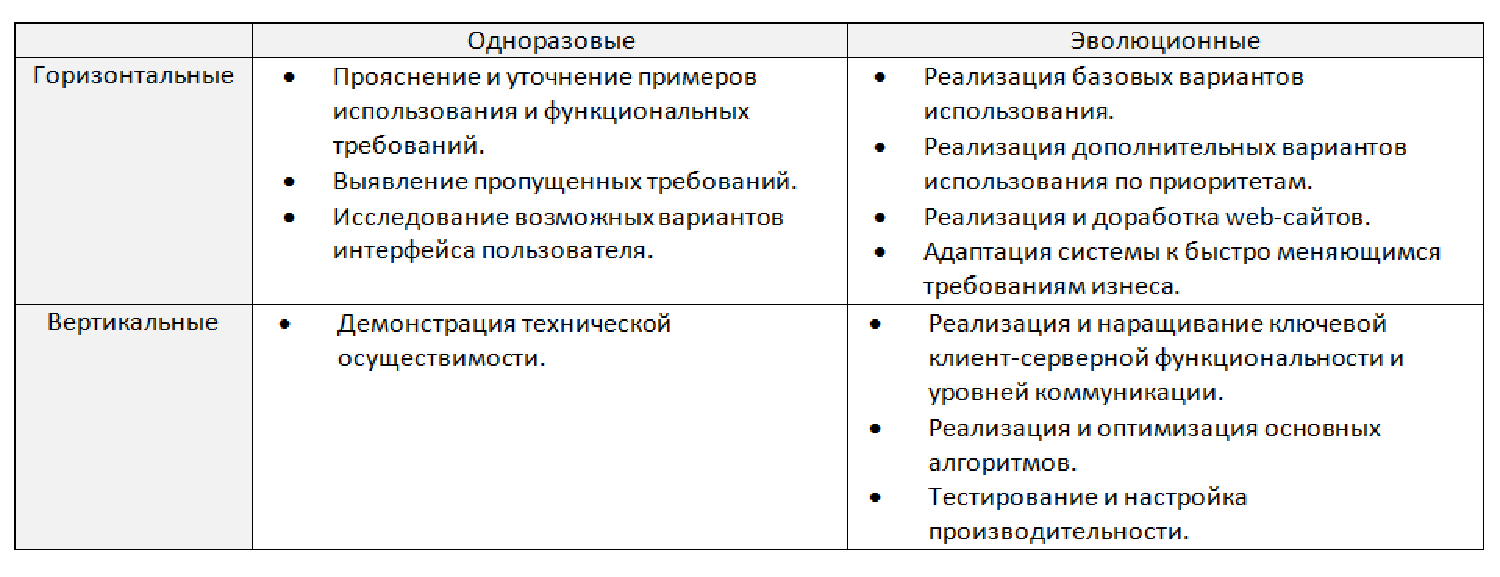
\includegraphics[width=1.2\textwidth]{pict8.pdf}}
\end{frame}

\lecturenotes

В таблице приведено соотношение между рассмотренными выше видами
прототипов~\cite[с.~55]{Maglinec}.


%%%%%%%%%%%%%%%%%%%%%%%%%%%%%%%%%%%%%%%%
\subsection{Проверка требований}
\begin{frame} \frametitle {Проверка требований}
\begin{itemize}
\item \alert{Verification} -- «проверка».
\item \alert{Validation} -- «проверка правильности», «аттестация»,
«утверждение».
\item Стандарт IЕЕЕ 1012-1986:
\begin{enumerate}
\item \alert{Верификация} -- процесс оценивания системы или
компонента с целью определить, удовлетворяют ли
результаты некой фазы условиям, наложенным в
начале данной фазы.
\item \alert{Валидация} -- процесс оценивания системы или
компонента во время или по окончании процесса
разработки с целью определить, удовлетворяет ли
она указанным требованиям.
\end{enumerate}
\end{itemize}

\end{frame}
\lecturenotes

Термин \alert{«верификация» (verification)} в русскоязычной литературе обычно
переводят, как «проверка». Термин \alert{«валидация» (validation)} - как «проверка правильности», «аттестация», «утверждение».

Согласно стандарту IЕЕЕ 1012-1986, верификация представляет собой процесс оценивания системы или компонента с целью определить, удовлетворяют ли
результаты некой фазы условиям, наложенным в начале данной фазы. Валидация в этом
же стандарте определяется, как процесс оценивания системы или компонента во время
или по окончании процесса разработки с целью определить, удовлетворяет ли она
указанным требованиям.

Отличие заключается в том, что: если
верификация связана с выяснением того, удовлетворяет ли разрабатываемый объект, либо
процесс его создания сформулированным требованиям, то валидация отвечает на вопрос –
правильно ли разработан целевой объект (продукт), удовлетворяет ли он потребностям
заказчика. Другой аспект валидации заключается в том, что она обычно увязывается с
формальной приёмкой (аттестацией) системы.

Усилия, прилагаемые в рамках
работ по верификации и валидации, направлены на обеспечение качества как
неотъемлемой характеристики программного обеспечения и удовлетворение
пользовательских требований~\cite[с.~64--65]{Maglinec}.

Проверка требований же гарантирует, что все положения требований корректны, отражают желаемые качественные характеристики и удовлетворяют потребностям клиента. Может оказаться, что требования, в спецификации требований к ПО выглядевшие превосходно, при реализации чреваты проблемами. В большинстве случаев удается выявить двусмысленности и неопределенности, написав для требований сценарии тестирования. Если требования должны стать надежной основой для проектирования и итоговой проверки системы посредством системного тестирования или тестирования на приемлемость для пользователей, эти проблемы необходимо устранить~\cite[с.~51]{Wiegers}.

%%%%%%%%%%%%%%%%%%%%%%%%%%%%%%%%%%%%%%%%%%%%%%%%
%новый слайд
\begin{frame} \frametitle {Определение критериев
приемлемости}

  \begin{block}{}
\alert{Критерии приемлемости} должны отразить точку зрения Заказчика на то, что он считает правильной системой, т.е. годится ли разработанное ПО для решения поставленных им задач.
	  \end{block}
		\begin{itemize}
\item Приём: делегирование разработки тестов на
приемлемость пользователям. 
\item Позволяет уже на этапе
сбора информации перейти от формулировки вопроса с
\alert{«Что вам нужно делать с помощью системы?»} к \alert{«Как вы
делаете вывод о том, что система удовлетворяет вашим
потребностям?»}.
\item Если клиент не может описать, как он оценит, что конкретное требование удовлетворено системой, значит, требование сформулировано недостаточно ясно.
\end{itemize}
\end{frame}


\lecturenotes

При формальной приёмке продукта существуют две типовые процедуры: демонстрация продукта Разработчиком на тестовых сценариях и проверка продукта Заказчиком.

Крайне важно, наряду с формированием требований, вовлечь Заказчика на ранних стадиях
создания продукта в процесс формирования критериев приемлемости. \alert{Критерии
приемлемости (acceptance criteria)} должны отразить точку зрения Заказчика на то, что он
считает правильной системой.

Делегирование разработки тестов на приемлемость пользователям — эффективная
стратегия разработки требований. Это позволяет уже на этапе сбора информации
перейти от формулировки вопроса с «Что вам нужно делать с помощью системы?» к «Как
вы делаете вывод о том, что система удовлетворяет вашим потребностям?». Если клиент
не может описать, как он оценит, что конкретное требование удовлетворено системой,
значит, требование сформулировано недостаточно ясно.

Раннее формирование тестов для проверки приемлемости позволяет обнаружить
дефекты в требованиях.
Проверка приемлемости базируется на ключевых (существенных) вариантах
использования. При этом следует абстрагироваться от альтернативных сценариев и
исключений и сосредоточить внимание на основном потоке событий. Необходимо учесть
также и нефункциональные требования, такие, как производительностью, легкость и
простота использования~\cite[с.~68]{Maglinec}.


%%%%%%%%%%%%%%%%%%%%%%%%%%%%%%%%%%%%%%%%%%%%%%%
\begin{frame} \frametitle {Критерии для проверки
требований}
\begin{itemize}
\item Требования должны удовлетворять
свойствам.
\item В спецификации требований к ПО должным
образом описаны предполагаемые
возможности и характеристики системы,
которые удовлетворят потребности
совладельцев.
\item Требования к ПО точно отражают системные
требования, бизнес-правила и др.
\item Требования обеспечивают качественную
основу для проектирования и сборки ПО.
\end{itemize}
\end{frame}

\lecturenotes

Так как критерием проверки ПО служат требования, то что может послужить критерием проверки самих требований? Ответ заключается в том, что
требования должны удовлетворять свойствам требований. Кроме того,
следует убедиться в том, что:
\begin{itemize}
\item в спецификации требований к ПО должным образом описаны предполагаемые
возможности и характеристики системы, которые удовлетворят потребности
различных заинтересованных в проекте лиц;
\item требования к ПО точно отражают системные требования, бизнес-правила и др.;
\item требования обеспечивают качественную основу для проектирования и сборки ПО~\cite[с.~64]{Maglinec}.
\end{itemize}


%%%%%%%%%%%%%%%%%%%%%%%%%%%%%%%%%%%%%%%%%%%%%%
\begin{frame} \frametitle {Проблемные ситуации}
\begin{itemize}
\item \alert{Двусмысленность требований}
\begin{itemize}
\item Такое требование может привести к различным его интерпретациям представителями Разработчика и Заказчика.
\end{itemize}
\item \alert{«Золочение» продукта}
\begin{itemize}
\item Ситуации, когда разработчики добавляют
функции, которых нет в спецификации, но им кажется, что это понравится пользователям.
\end{itemize}
\item \alert{Минимальная спецификация}
\begin{itemize}
\item Ситуации, когда у проекта не создана полная документация требований, имеется лишь некий набросок требований.
\end{itemize}
\item \alert{Пропуск типов пользователей}
\begin{itemize}
\item Представитель Разработчика должен объективно оценить организационную структуру предприятия и его бизнес-процессы.
\end{itemize}
\end{itemize}
\end{frame}

\lecturenotes

Предотвращение ошибок в требованиях и обнаружение их на ранних стадиях сильно уменьшает объем переделки~\cite[с.~16]{Wiegers}. Дефекты в требованиях представляют собой угрозу успеху проекта, где успех означает выпуск продукта, который удовлетворяет ожиданиям пользователей в качестве и функциональности при соблюдении бюджета и графика проекта~\cite[с.~17]{Wiegers}.

\alert{Двусмысленность требований}

Один из ее симптомов — пользователь имеет возможность интерпретировать одно и то же положение по-разному. Другой — что у нескольких читателей требований возникает разное
представление о продукте. Кроме того, двусмысленность зачастую
проистекает из неточности и плохой детализации требований, в результате чего разработчикам приходится заполнять возникающие
пробелы собственными силами.

Один из способов обнаружить двусмысленности — пригласить различных представителей пользователей для официальной экспертизы требований. Другой способ вскрыть двусмысленность — написать вариант тестирования для требования и построить прототип~\cite[с.~18]{Wiegers}.

\alert{«Золочение» продукта}

Под «золочением» понимают такие ситуации, когда разработчики добавляют функции, которых нет в спецификации, но им кажется, что это понравится пользователям. Зачастую же клиентам не нужны такие избыточные возможности, получается, что время, отведенное на реализацию тратится впустую.

Прежде чем просто вставлять новые функции,
разработчики и аналитики должны представить свои творческие идеи на суд заказчиков. Задача команды — четко соблюдать требование спецификации, а не действовать за спиной клиентов без одобрения.

Пользователи иногда требуют функции или элементы интерфейса, которые выглядят отлично, но не представляют особой ценности для продукта. Все, что вы захотите добавить, стоит времени и денег, поэтому постарайтесь осознать ценность своевременного выпуска продукта. 

Чтобы уменьшить «золочение», отслеживайте каждый бит функциональности до его первоисточника, чтобы четко понимать, почему именно он включен в продукт. Применение вариантов использования
для извлечения требований поможет сосредоточиться на выборе тех элементов, которые помогут пользователям выполнять их бизнес-задачи~\cite[с.~18-19]{Wiegers}.

\alert{Минимальная спецификация}

Иногда сотрудников отдела маркетинга или менеджеров охватывает искушение создать урезанный вариант спецификации, как, например набросок концепций продукта на салфетке. Они ожидают, что разработчики «нарастят» спецификацию на основе этих набросков, пока проект развивается. Это годится для тесно сплоченной команды, которая занимается небольшой системой, или когда выполняется проект-исследование, или когда требования действительно гибкие (McConnell, 1996). Хотя в большинстве случаев это все-таки плохой вариант для разработчиков (которые могут действовать при некорректных предположениях и с ограниченными инструкциями), а также дезориентирует клиентов (которые не получат тот продукт, который они воображали)~\cite[с.~19]{Wiegers}.

\alert{Пропуск классов пользователей}

Большинство продуктов предназначены для нескольких групп пользователей, которые могут применять различные наборы функций с разной частотой и имеют опыт работы с ПО самого широкого диапазона.

Если не были определены важные классы пользователей для продукта заранее, некоторые потребности клиентов не будут учтены.
После идентификации всех классов необходимо удостовериться, что каждый из них имеет голос~\cite[с.~19]{Wiegers}.

%%%%%%%%%%%%%%%%%%%%%%%%%%%%%%%%%%%%%%%%%%%%%%

\begin{frame} \frametitle {Проблемные ситуации}
\begin{itemize}

\item \alert{Небрежное планирование} 
\begin{itemize}
\item При плохо просчитанной смете проект больше всего страдает из-за затрат на частые изменения требований, пропущенных требований, недостаточного взаимодействия с пользователями, недетализированной спецификации требований и плохого
анализа.
\end{itemize}

\item \alert{«Разрастание» требований пользователей}
\begin{itemize}
\item Так как требования тщательно прорабатываются и их объем со временем увеличивается, проект часто выходит за установленные рамки как по срокам, так и по бюджету. 
\end{itemize}

\item \alert{Недостаточное вовлечение пользователей}
\begin{itemize}
\item  Трудно добраться до
людей, которые непосредственно будут иметь дело с продуктом, а выразители мнения пользователей не всегда понимают, что тем нужно в реальности. 
\end{itemize}

\end{itemize}
\end{frame}

\lecturenotes


\alert{Небрежное планирование}

Неопределенные, недетализированные требования порождают слишком оптимистические оценки: они «выходят боком», когда возникает перерасход.

При плохо просчитанной смете проект больше всего страдает из-за затрат на частые изменения требований, пропущенных требований, недостаточного взаимодействия с пользователями, недетализированной спецификации требований и плохого
анализа (Davis, 1995)~\cite[с.~20]{Wiegers}.

\alert{«Разрастание» требований пользователей}

Так как требования тщательно прорабатываются и их объем со временем увеличивается, проект часто выходит за установленные рамки как по срокам, так и по бюджету. 

Первоначально принятые планы не всегда основаны на реалистичном понимании размера и сложности требований, ограничение же на модификацию только усиливает проблемы.Эти проблемы частично кроются в частых запросах пользователей на изменения, а частично — в том, какими способами разработчики отвечают на них.

Чтобы управлять границами требований, для начала нужно уточнить бизнес-цели проекта, основы его образа, рамки, ограничения, критерии успеха и ожидаемую пользу. Необходимо оценить, как предполагаемые характеристики или изменения требований отразятся на связанной с ними структуре. Эффективный процесс модификации заставляет интенсивнее работать аналитиков, которые помогут всем заинтересованным
лицам принять обдуманные бизнес-решения относительно того, какие изменения следует принять, и увязать их стоимость со временем, ресурсами или возможными компромиссами. Изменения зачастую критически важны для успеха, однако они всегда имеют цену.

По мере того как продукт модифицируется в процессе разработки, его архитектура может медленно разрушаться. «Заплатки» кода затрудняют понимание и поддержку продукта. Добавление кода может стать причиной нарушения твердых и взаимосвязанных принципов дизайна и разрыва связей (McConnell, 1993). 

Чтобы минимизировать
возможность потери качества продукта в результате проблем такого рода, вначале тестируют, как возможные изменения отразятся на архитектуре и дизайне, а затем уже их реализуют непосредственно
в коде~\cite[с.~17-18]{Wiegers}.

\alert{Недостаточное вовлечение пользователей}

Заказчики зачастую не понимают, почему так важно тщательно собрать требования и обеспечить их качество. Разработчики не всегда придают значение вовлечению пользователей в процесс. В любом случае трудно добраться до
людей, которые непосредственно будут иметь дело с продуктом, а выразители мнения пользователей не всегда понимают, что тем нужно в реальности. 

Недостаточное вовлечение пользователей ведет к обнаружению ошибок в требованиях на поздних стадиях проекта, а значит, к задержке завершения проекта. Нет альтернативы сотрудничеству
разработчиков непосредственное реальными пользователями на протяжении всего проекта~\cite[с.~17]{Wiegers}.

%%%%%%%%%%%%%%%%%%%%%%%%%%%%%%%%%%%%%%%%%%%%%%
\begin{frame} \frametitle {Методы проверки требований}
  \begin{block}{}
\alert{Проверка требований} гарантирует, что все их положения корректны, отражают желаемые качественные характеристики и удовлетворяют потребностям клиента.
  \end{block}
\begin{itemize}
\item \alert{по широте анализа} – просмотр (выборочная проверка) и сквозной контроль (тотальная
проверка);
\item \alert{по степени формализации} – неофициальные процедуры, процедуры, проводимые по
формальным правилам (инспекции, экспертизы);
\item \alert{по составу группы проверки} – с (без) участием автора, с (без) участием менеджера
проекта, с (без) участием представителей внешних организаций;
\item \alert{по используемым средствам} – тексты требований, тестовые сценарии, критерии
приемлемости, прототипы.

\end{itemize}
\end{frame}

\lecturenotes

Существует значительное количество методов и средств проверки требований, они отличаются по ряду параметров. Некоторые другие, наиболее важные из перечисленного выше, методы и средства, рассмотрены далее.


\begin{frame} \frametitle {Методы проверки требований}

\begin{itemize}
\item \alert{Неофициальные просмотры требований}
\begin{itemize}
\item Просмотр «за столом», коллективная проверка, критический анализ.
\end{itemize}

\item  \alert{Инспекции}
\begin{itemize}
\item Базируется на своде формальных требований и правил.
Общим инструментом, используемым при инспектировании, является проверочный лист
(checklist), содержащий аномалии и вопросы,
связанные с аспектами, вызывающими интерес.
\end{itemize}

\item  \alert{Разработка тестов}
\begin{itemize}
\item Тестовые сценарии (ТС) рекомендуется создавать уже на ранних стадиях работы с требованиями, в идеале – после получения запросов совладельцев, параллельно с разработкой вариантов использования.
\end{itemize}
\end{itemize}
\end{frame}

\lecturenotes

\alert{Неофициальные просмотры требований}

Различают несколько способов неофициальных просмотров требований:
\begin{itemize}
\item просмотр «за столом»,
\item коллективная проверка,
\item критический анализ.
\end{itemize}

В первых двух случаях автор требований обращается за помощью к коллегам (соответственно, к одному, либо к нескольким) с целью выдачи практических
рекомендаций по улучшению продукта. В третьем случае автор осуществляет презентацию разработанные им требования на совещании с последующим обсуждением. Неофициальные просмотры используют для знакомства с разработкой, сбора
отзывов, формирования обратной связи. По статистике
неофициальные просмотры позволяют выявить до 60\% ошибок в требованиях~\cite[с.~66-67]{Maglinec}.

\alert{Инспекции}

Понятие инспекции, применительно к IT-индустрии, впервые было сформулировано Майклом Фэганом (Michael Pagan) из IBM в середине 70-х гг.19.
Согласно стандарту IEEE20, проведение инспекций, в отличие от неформальных просмотров, базируется на своде формальных требований и правил. 

Лица, занимающие управленческие позиции (менеджеры) в отношении к любым членам команды инспектирования, не должны участвовать в инспекциях.
Инспекция должна вестись под руководством непредвзятого (независимого от
проекта и его целей) лидера, обученного техникам инспектирования. Инспектирование всегда вовлекает авторов промежуточного или конечного
продукта.

Члены команды инспектирования могут специализироваться в различных
областями экспертизы (обладать различными областями компетенции), например,
предметной области, методах проектирования, языке и т.п. 

В заданный момент (промежуток) времени инспекции проводятся в отношении отдельного небольшого
фрагмента продукта (в большинстве случаев, фокусируясь на отдельных функциональных
или других характеристиках; часто, отталкиваясь от отдельных бизнес-правил,
функциональных требований или атрибутов качества, прим. автора). Каждый член
команды должен исследовать оцениваемый продукт и другие входные данные до
проведения инспекционной встречи, применяя, возможно, те или иные аналитические
техники в небольшим фрагментам продукта или к продукту, в целом, рассматривая в
последнем случае только один его аспект, например, интерфейсы.

Любая найденная
аномалия должна документироваться, а информация передаваться лидеру инспекции. В
процессе инспекции лидер руководит сессией и проверяет, что все подготовились к
инспектированию. Общим инструментом, используемым при инспектировании, является
проверочный лист (checklist), содержащий аномалии и вопросы, связанные с аспектами,
вызывающими интерес. Результирующий лист часто классифицирует аномалии и
оценивается командой с точки зрения его завершенности и точности~\cite[с.~67]{Maglinec}.

\alert{Разработка тестов}

Механизм вариантов использования (uses cases), 
позволяет ответить на вопрос: как будет использоваться система. Чтобы проверить
систему, используется аналогичный механизм: тестовых сценариев (test cases).

Тестовые сценарии (ТС) рекомендуется создавать уже на ранних стадиях работы с
требованиями, в идеале – после получения запросов совладельцев, параллельно с
разработкой вариантов использования. Тестовые сценарии, как и варианты использования, могут поддерживать разные
уровни абстракции. Различаются концептуальные и детальные ТС. Концептуальный
уровень предполагает проработку процедуры тестирования, инвариантную к конкретной
реализации UI.~\cite[с.~67--68]{Maglinec}.

%%%%%%%%%%%%%%%%%%%%%%%%%%%%%%%%%%%%%%%%%%%%%%
%новый слайд
\begin{frame} \frametitle {Тестирование требований с
помощью тестовых сценариев}
\begin{enumerate}
\item Построить матрицу, где по вертикали отмечены
функциональные требования, а по горизонтали –
тестовые сценарии.
\item Убедиться, что каждый из ТС осуществим на
существующем наборе требований.
\item Убедиться, что для каждого требования
представлен как минимум один ТС.
\item Прочертить «путь» каждого из ТС на карте
диалогов. Это позволит: обнаружить некорректные
или пропущенные требования, исправить ошибки на
карте диалогов и отшлифовать варианты
тестирования.
\end{enumerate}
\end{frame}

\lecturenotes

Как использовать тестовые сценарии для тестирования требований? К. Вигерс
предлагает следующую процедуру.

\begin{enumerate}
\item Построить матрицу, где по вертикали отмечены функциональные требования, а
по горизонтали – тестовые сценарии.
\item Убедиться, что каждый из ТС осуществим на существующем наборе требований.
\item Убедиться, что для каждого требования представлен как минимум один ТС.
\item Прочертить «путь» каждого из ТС на карте диалогов. Это позволит: обнаружить
некорректные или пропущенные требования, исправить ошибки на карте диалогов и
отшлифовать варианты тестирования.
\end{enumerate}

 На основе пользовательских требований
создаются сценарии функционального тестирования и документируется ожидаемое поведение продукта в конкретных условиях. Совместно с клиентами необходимо изучить сценарии тестирования и убедиться, что они отражают нужное поведение системы. Так же нужно проследить связь сценариев тестирования с функциональными требованиями и удостовериться,
что ни одно требование не пропущено и что для всех требований есть соответствующие сценарии тестирования~\cite[с.~52]{Wiegers}. 

Как быть с тестированием нефункциональных требований? Процедура анализа требований считается выполненной только тогда, когда все
требования, включенные в спецификацию, обладают методами оценки соответствия им
создаваемого программного продукта.
Для того, чтобы нефункциональные требования были измеримы, каждому из них в
идеале необходимо сопоставить количественную метрику. Если это не удаётся –
возможно, требование следует переформулировать, либо детализировать~\cite[с.~68]{Maglinec}.



\begin{frame} \frametitle {Вопросы к семинару}

\end{frame}

\begin{frame} \frametitle {Задание к семинару}
 
\end{frame}


\begin{thebibliography}{99}
\bibitem{Wiegers} Вигерс Карл, Разработка требований к программному обеспечению / Пер, с англ. — М.: Издательсш-торговый дом «Русская Редакция», 2004. —576с.: ил.
\bibitem{Maglinec} \href{http://ivan-shamaev.ru/wp-content/uploads/2013/06/Information-systems-analysis-and-requirements-analysis.pdf}{Анализ требований к информационным системам. Учебное пособие, Маглинец Ю.А., 2007}
\end{thebibliography}

\end{document}

%%% Local Variables: 
%%% mode: TeX-pdf
%%% TeX-master: t
%%% End: 
